\chapter{PMT Upgrade}

\begin{figure}
	\centerline{
		\mbox{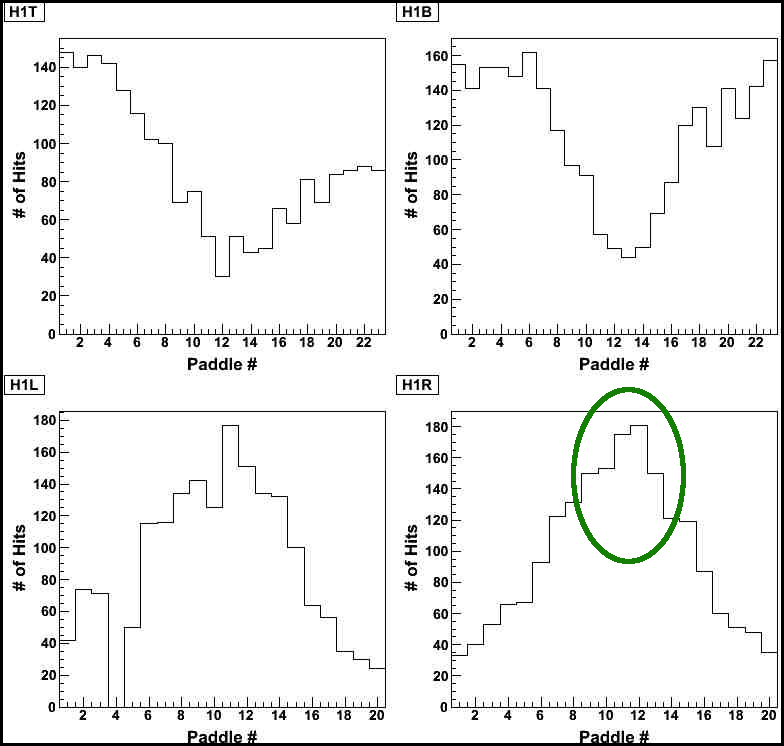
\includegraphics[width=0.5\textwidth]{figures/nosag.jpg} 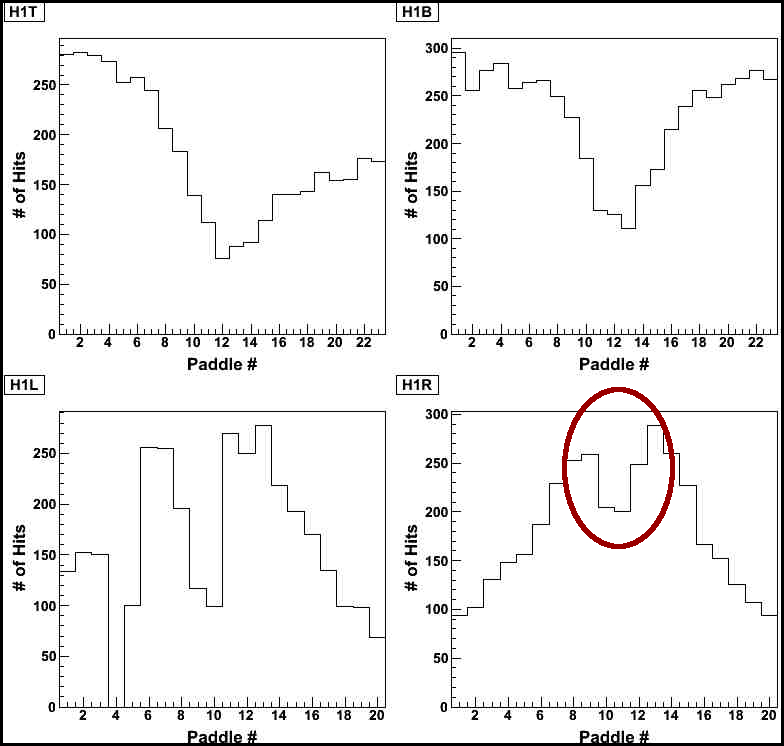
\includegraphics[width=0.5\textwidth]{figures/sag.jpg}}
	}
	\caption{(Left) Histogram of hodoscope `hits' in a typical event; (Right) Histogram of high-intensity event, with marked sagging most noticeably in the middle of the y-measuring hodoscopes}
	\label{fig:sag}
\end{figure}

During Run I of SeaQuest, observations of hodoscope wire maps (as in Fig.~\ref{fig:sag}) suggested an apparent drop in expected performance in the $y-$measuring hodoscopes. While this performance was most obviously seen in the $y-$measuring hodoscope planes, the $x-$measuring planes were likely also affected. This effect was assumed to be due to high-intensity RF buckets that caused very high multiplicity in all of the detectors in the spectrometer for that event. The result of these intense events seemed to push the PMTs and/or their PMT base electronics past their operational capacity.

The understood cause of this \emph{``sag''} in performance, as it came to be called, was due to a destabilization in the voltage divider in the PMT base. This critical component holds each dynode stage at a specific voltage, and when this destabilizes and is unable to maintain an appropriate voltage difference between dynode stages, inefficient performance of the PMT results.

During the Fall of 2012, prototyping and testing was performed with the goal in mind being to assemble a new base for the Philips XP-2008 PMTs~\cite{tubespecs} and compare its performance to the original PMT base and to some modern, high-performance Hamamatsu PMTs. Once a base design tested well, the new bases would be manufactured and installed in the existing frames of the original PMT bases.

\section{PMT Basic Construction and Operation}

\begin{figure}
	\centering
	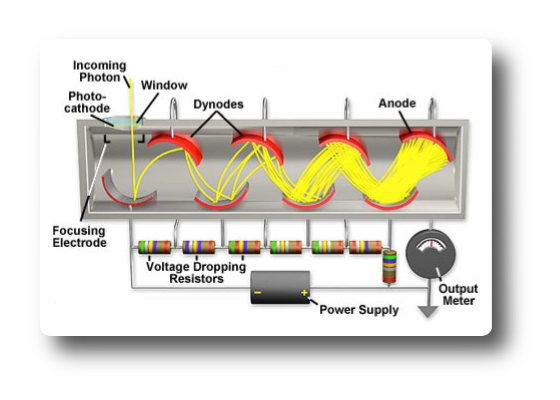
\includegraphics[width=0.5\textwidth]{figures/pmt-diagram.png}
	\caption{A diagram of typical PMT operation. The circuit controlling the voltage-dropping resistors is the part that was upgraded in this chapter.}
	\label{fig:pmt}
\end{figure}

Figure~\ref{fig:pmt} shows a schematic design of a typical photomultiplier tube and base setup. It consists of a photocathode that is followed by an electron multiplier section (or dynode string) then an anode from which a final signal is delivered. During operation, a high voltage is applied to the photocathode, dynodes, and anode in such a way that there's a potential ``ladder'' going from stage to stage. When an incident photon from the hodoscope scintillator paddle hits the photocathode, an electron is emitted via the photoelectric effect. The voltage difference between the cathode and dynode stages draws the emitted electron to the dynodes, and each time an electron hits a dynode, some of that electron's energy is transferred to other electrons in the dynode. These electrons then are emitted and become accelerated towards the next dynode stage. This process is called secondary emission, and by the time the process is repeated, there is a cascade or avalanche of electrons that land on the anode, resulting in a signal that can be amplified and analyzed.

It is the case that the voltage divider ultimately supplies the electrons that are emitted in this signal cascade. If too many photons and resultant electron cascades occur, the dynode stages' voltage divider will destabilize as they attempt to resupply the the dynode stages with electrons. The problem that was experienced at SeaQuest was that these high-intensity events were flooding the PMTs with photons, causing this ``saturation'' which caused this destabilization and the inefficient performance that was observed. The goal specifically was to test out modern base designs that provided for added stability to the performance of the voltage divider, even under high rates.

In general, each base divides around a \unit[-1500]{V} potential total over the photocathode (K), ten dynode stages (D1-D10), and the anode (A). There are two currents that are referred to here:
\begin{itemize}
	\item Signal Current: This is the signal that passes over the anode, which is the end-result of the cascading secondary emission electrons from each dynode stage.
	\item Bleeder Current: This is the current through the voltage divider. It is termed the ``bleeder'' current since the compounding electrons in the signal current must be ``bled'' from the current through the voltage divider.
\end{itemize}

Throughout these voltage base designs, capacitors are commonly implemented in the latter dynode stages where the most electrons are emitted. These capacitors, when charged, are able to replenish the lost charge on its corresponding dynode stage in the event that an intense light pulse induces a large signal current.  As the capacitor is able to hold its own chare, this resupply can occur without requiring the charges to be drawn from the bleeder current, thereby keeping the voltage across the dynode stages more stable.

\section{PMT Base Design Iterations}

There were several iterations of base design to determine which was best to approach for full base production and installation. The core addition was the inclusion of transistors

\subsection{Original Base}

This is the PMT base that is currently used with our XP-2008 PMT's. It features capacitors of increasing capacitance along the last six stages, and steadily increases the voltage across the final four stages.

\begin{figure*}[h]
	\centerline{
		\mbox{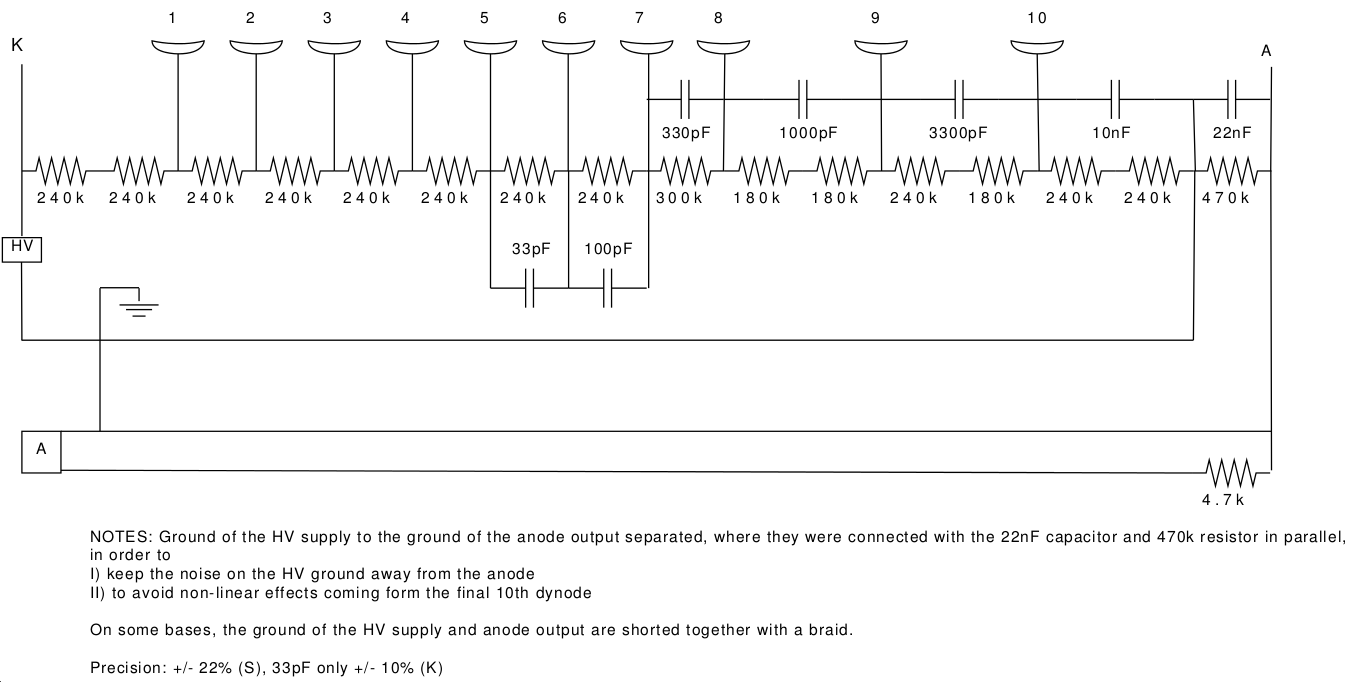
\includegraphics[width=0.75\textwidth]{figures/pmt.png}}
	}
	\caption{The original PMT base design.}
	\label{fig:original-board}
\end{figure*}

\begin{figure*}[h]
	\centerline{
		\mbox{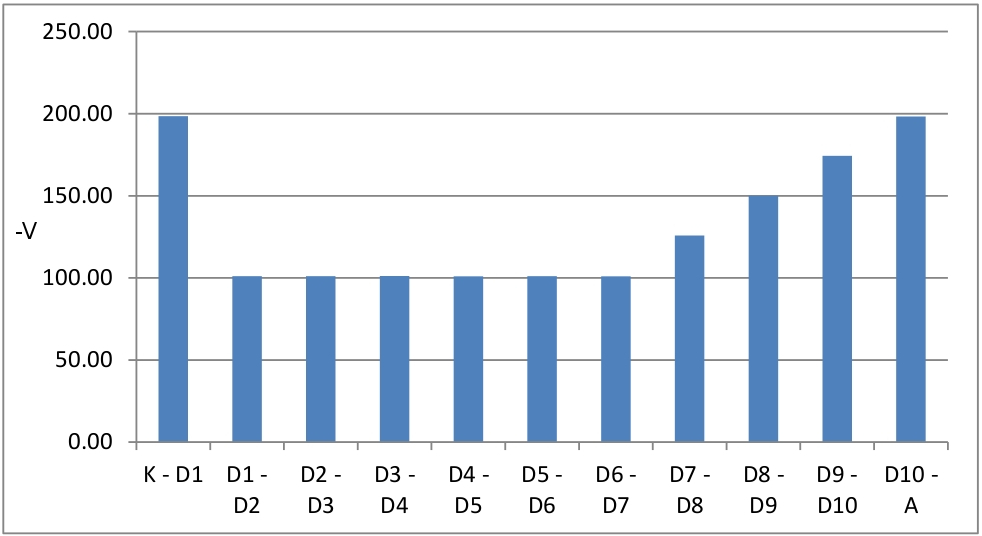
\includegraphics[width=0.75\textwidth]{figures/original-volt.jpg}}
	}
	\caption{The (negative) voltage between subsequent stages for the original PMT base.}
	\label{fig:original-volt}
\end{figure*}

\subsection{Prototype Base v1}

This is the base design provided by Sten Hansen (Fermilab Particle Physics Division), designed in 2010 for the same model of PMT's for use at CERN. 

Three important features of this design include:

\begin{itemize}
	\item
	Lower resistance
	\item
	Parallel currents
	\item
	Transistors and diodes
	\item
	(More) Even distribution of voltage
\end{itemize}

The lower overall resistance of the voltage divider increases the bleeder current. This means that the base will be more capable of handing high-intensity/-rate events, as it will be better able to replenish the charges on each dynode stage in the case of a large signal. Typically, the larger the bleeder current, the larger the signal current can be without destabilizing the voltage divider.

At dynode six on Figure \ref{fig:v1-board}, we see that the current is split into two paths. The intent here is for the smaller current that goes through the series of $1M\Omega$ resistors maintains the voltage difference, and the larger current that freely passes through the transistors supplies the dynode stages with needed charge.

Transistors are introduced here to maintain the proper voltage division. If at any point the proper voltage drop across the gates of the transistors is not supplied (and thereby across the dynode stages), the source-to-drain current through the transistor is stopped until the proper gate voltage is restored. This helps to regulate the voltage across the dynodes, but if the charges lost to the signal current are not restored, the PMT will still eventually "sag" and fail.

The diodes are there to prevent the current from moving across the transistors improperly, and thereby preventing them from being damaged when powering the circuit on and off.

Also, the voltage across each stage, from D1 to A, are relatively flat. According to the specifications for the Philips XP-2008 photomultiplier tube, this is the recommended voltage configuration for maximum gain \cite{tubespecs}.

\begin{figure*}[h]
	\centerline{
		\mbox{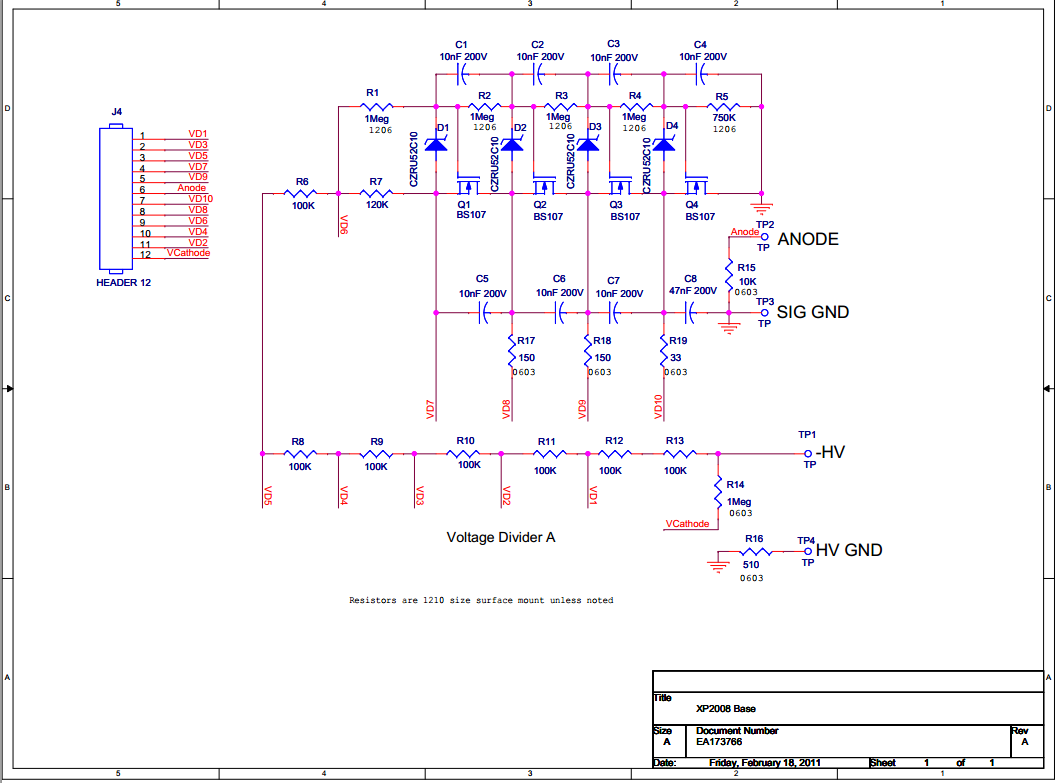
\includegraphics[width=0.7\textwidth]{figures/newbase.png}}
	}
	\caption{The Prototype v1 board.}
	\label{fig:v1-board}
\end{figure*}

\begin{figure*}[h]
	\centerline{
		\mbox{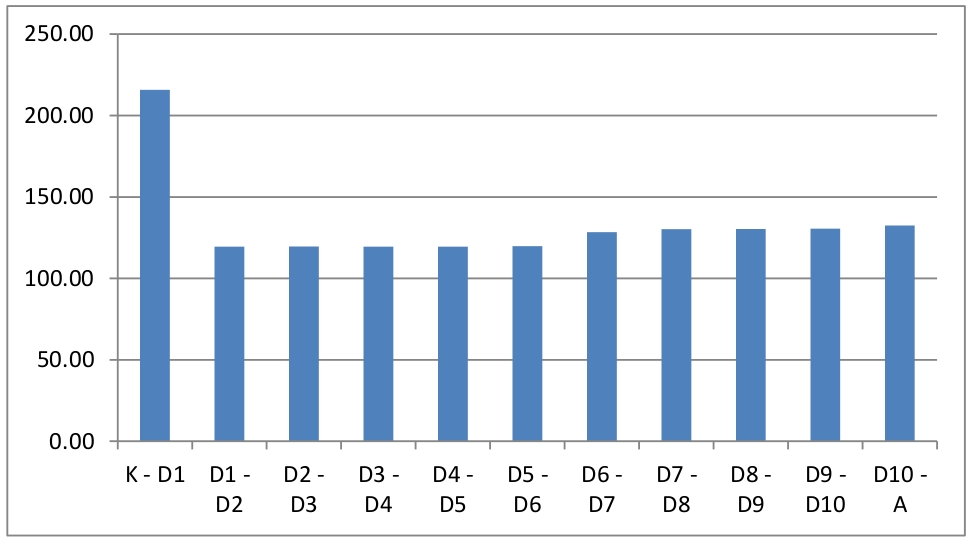
\includegraphics[width=0.75\textwidth]{figures/v2-volt.jpg}}
	}
	\caption{The (negative) voltage between subsequent stages for the Prototype v1 PMT base.}
	\label{fig:v1-volt}
\end{figure*}
\newpage

\subsection{Prototype Base v2}

The first modification made to the prototype board was to simply halve the resistance of each of the first six stages (R6-R13 on Fig. \ref{fig:v1-board}) to increase the bleeder current.

\begin{figure*}[h]
	\centerline{
		\mbox{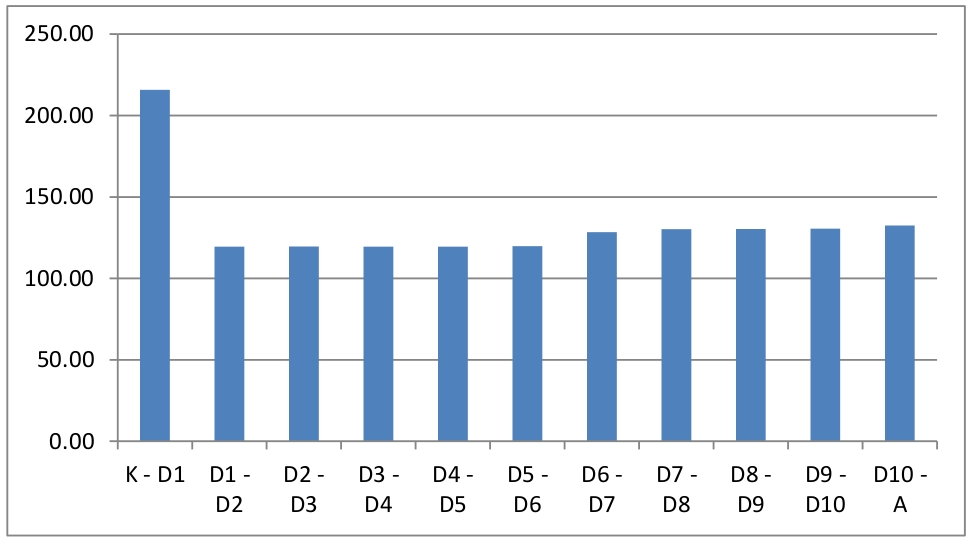
\includegraphics[width=0.75\textwidth]{figures/v2-volt.jpg}}
	}
	\caption{The (negative) voltage between subsequent stages for the Prototype v2 PMT base.}
	\label{fig:v2-volt}
\end{figure*}
\newpage

\subsection{Prototype Base v3}

This modification "transistorized" the D5-D6 and D6-D7 stages in the case that the destabilization was occurring even at these earlier stages (Figure \ref{fig:v3-board}).

\begin{figure*}[h]
	\centerline{
		\mbox{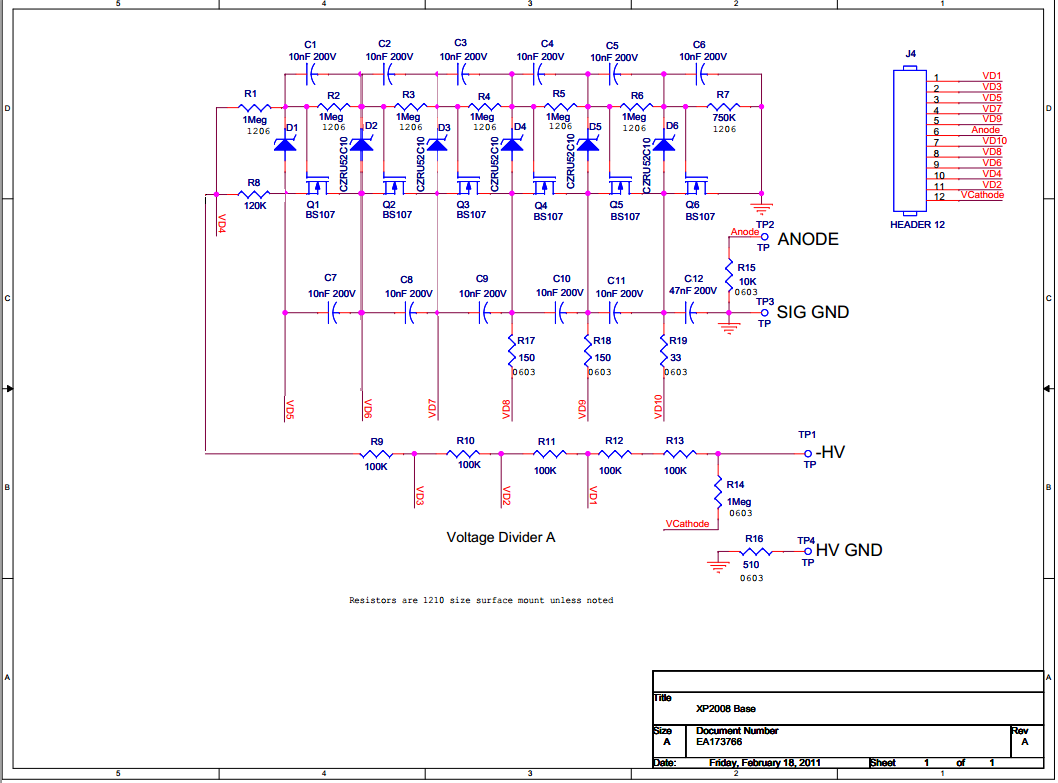
\includegraphics[width=0.75\textwidth]{figures/newbase_6mosfet.png}}
	}
	\caption{The Prototype v3 board: 3 more transistorized stages than the Prototype v1 design.}
	\label{fig:v3-board}
\end{figure*}

\begin{figure*}[h]
	\centerline{
		\mbox{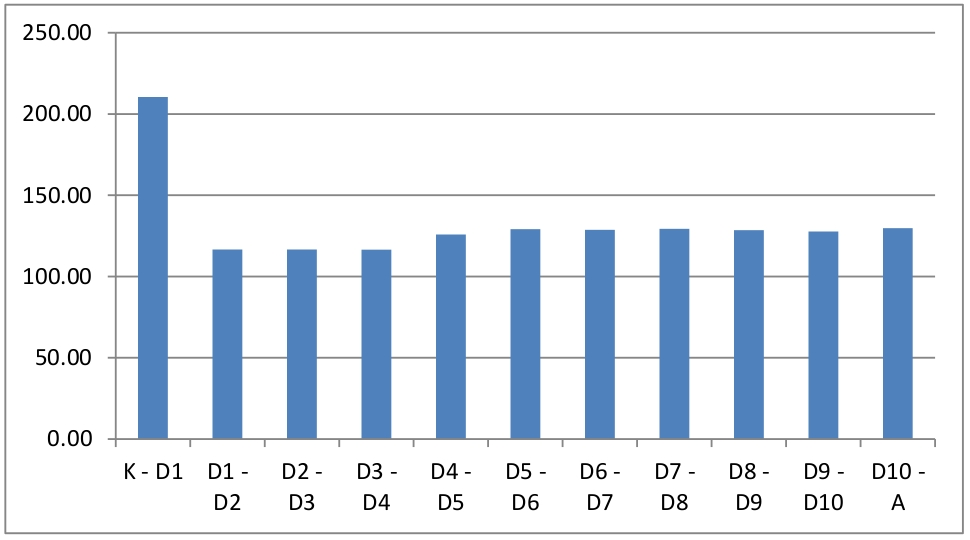
\includegraphics[width=0.75\textwidth]{figures/v3-volt.jpg}}
	}
	\caption{The (negative) voltage between subsequent stages for the Prototype v3 PMT base.}
	\label{fig:v3-volt}
\end{figure*}
\newpage
\subsection{Prototype Base v4}

Here, the resistance over the final stage (D10-A) was increased from $1M\Omega$ to $1.5M\Omega$ (R5 in Figure \ref{fig:v1-board}). This was done in case that the final batch of electrons needed help being "swept" to the anode with a higher voltage difference.

\begin{figure*}[h]
	\centerline{
		\mbox{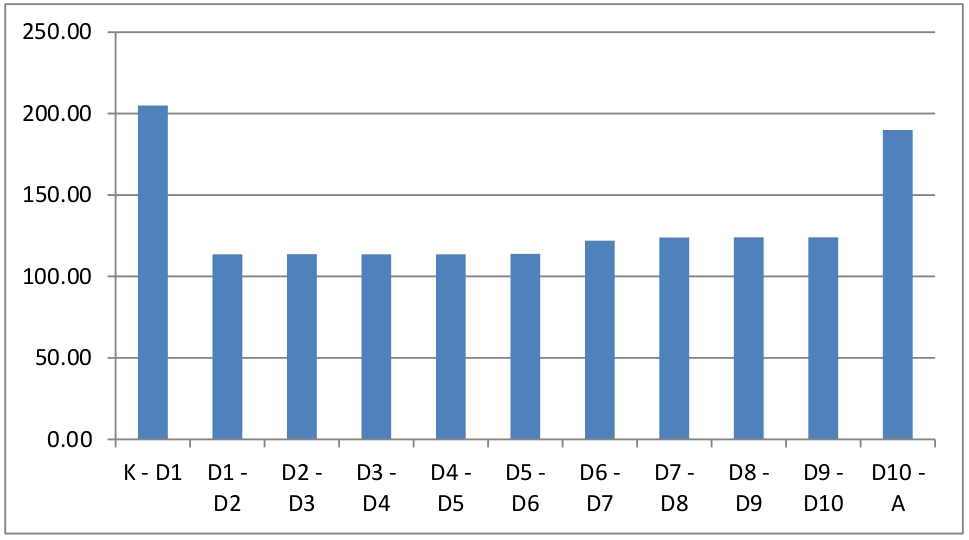
\includegraphics[width=0.75\textwidth]{figures/v4-volt.jpg}}
	}
	\caption{The (negative) voltage between subsequent stages for the Prototype v4 PMT base.}
	\label{fig:v4-volt}
\end{figure*}
\newpage

\section{PMT Base Comparisons}

There is a specific difficulty with the objective to increase the rate capability of our PMT's. This difficulty is that we do not have a target rate to attain. The rate and intensity that caused the original PMT+base to sag is unknown, and if it was known, it would be difficult to match the intensity with an experimental setup.

As a result, the objective in these tests is to \emph{compare} the performance of the same PMT using different bases.

\subsection{Testing Apparatus and Measurments}

In this experiment, a PMT attached to a PMT base is placed into a light-tight box along with an fast-pulsing LED. 

The LED is driven by an Agilent function generator capable of generating signals up to 30MHz. The LED's intensity is attenuated by a neutral density filter (NDF), with a rating D=3.0, where the NDF allows 1 in $10^D$ photons through (1 in 1000 for D=3.0).

The PMT base is powered by a high voltage supply with an ammeter between the two in order to measure the bleeder current. The PMT signal is processed 

\begin{figure*}[h]
	\centerline{
		\mbox{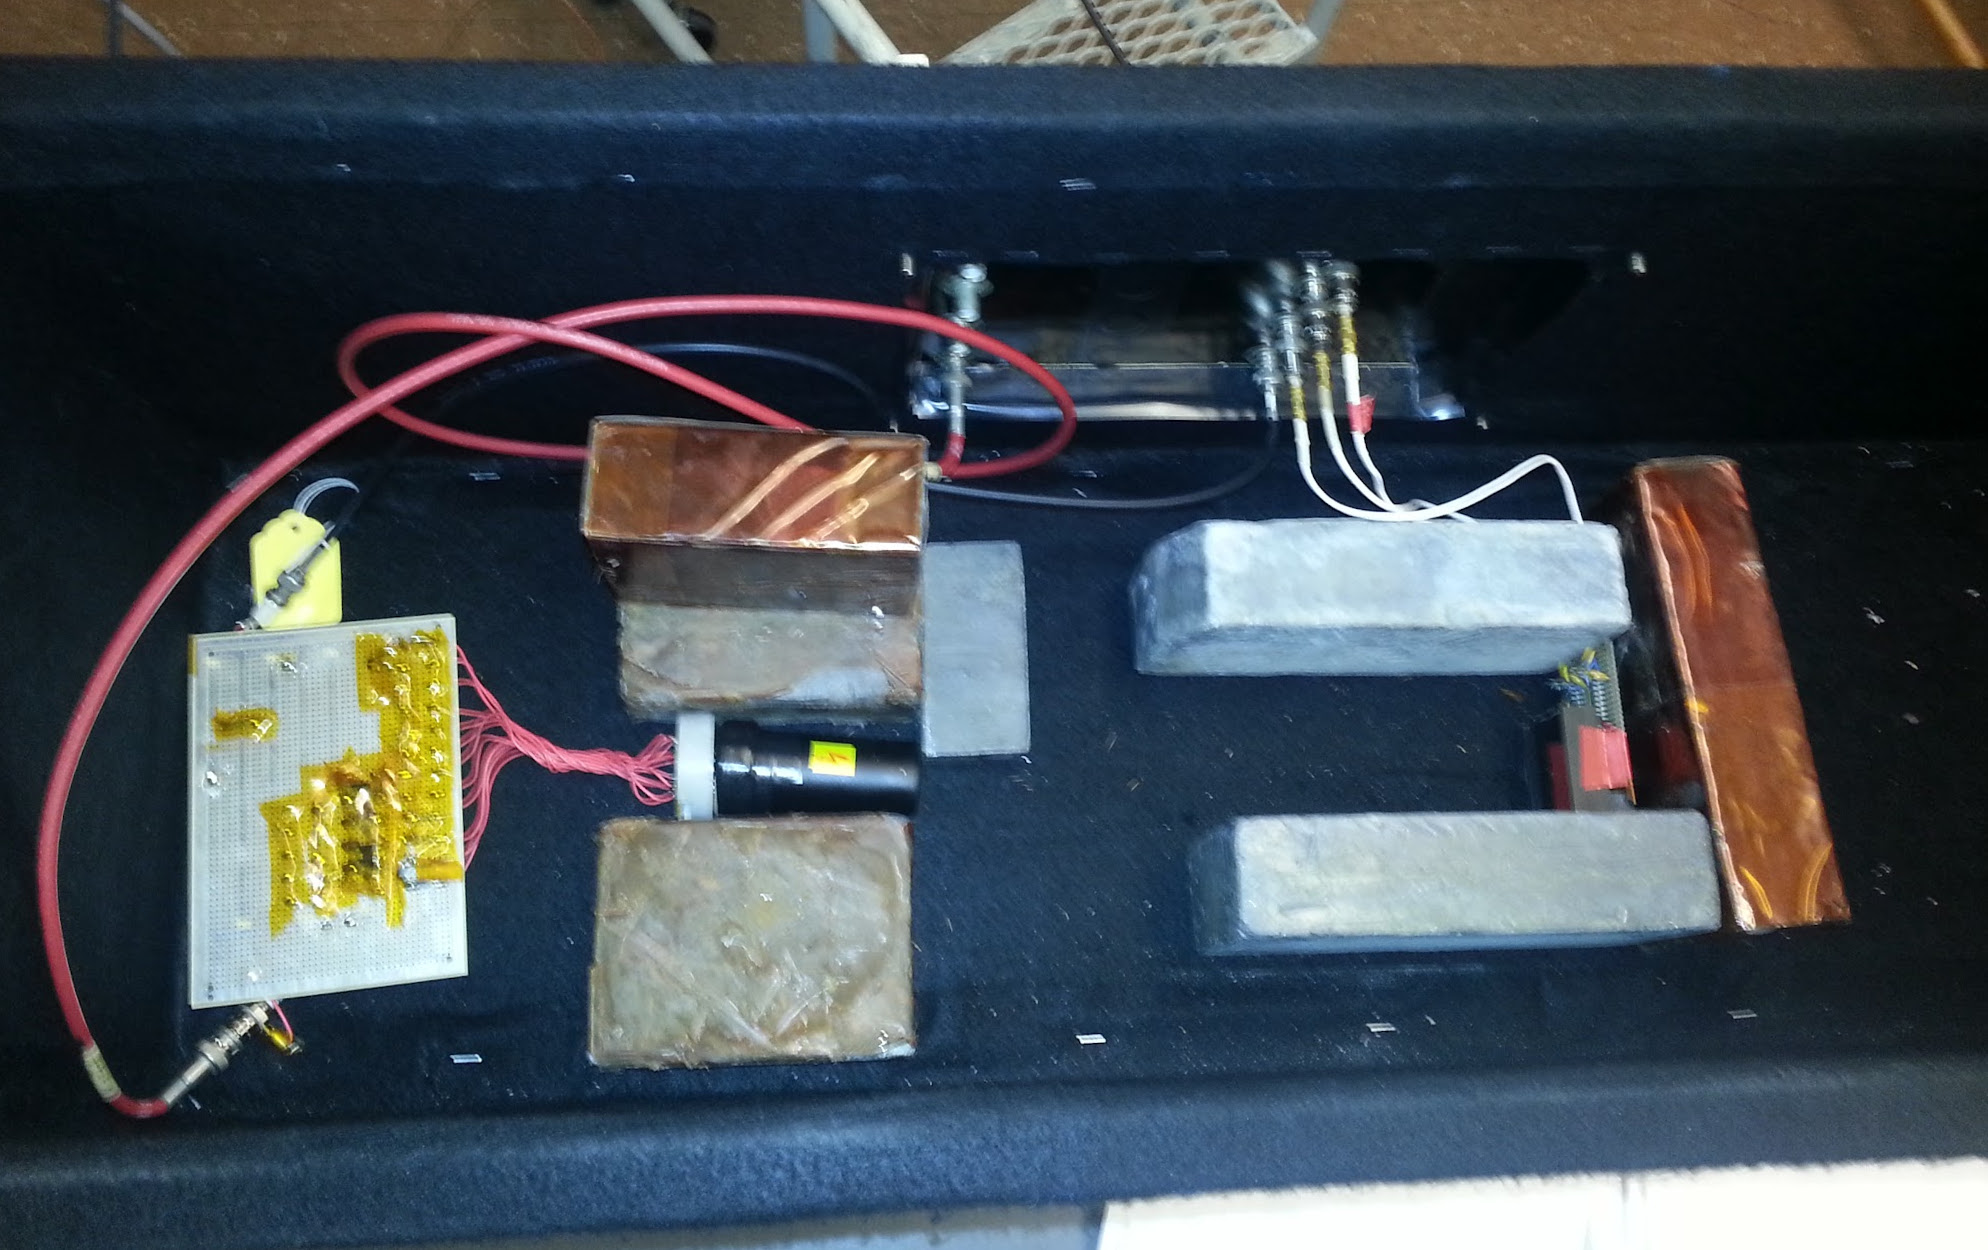
\includegraphics[width=0.75\textwidth]{figures/setup.jpg}}
	}
	\caption{Inside of a lightbox, we have our prototype board (left) wired up to a Philips XP-2008 PMT (middle), facing a fast-led source (right) }
	\label{fig:setup}
\end{figure*}
